\documentclass{article}


% if you need to pass options to natbib, use, e.g.:
    \PassOptionsToPackage{numbers, compress}{natbib}
% before loading neurips_2024


% ready for submission
% \usepackage{neurips_2024}
% \newcommand{\anon}[1]{\censor{#1}}


% to compile a preprint version, e.g., for submission to arXiv, add add the
% [preprint] option:
   \usepackage[preprint]{neurips_2024}
   \newcommand{\anon}[1]{{#1}}


% to compile a camera-ready version, add the [final] option, e.g.:
%    \usepackage[final]{neurips_2024}
%    \newcommand{\anon}[1]{{#1}}

% to avoid loading the natbib package, add option nonatbib:
%    \usepackage[nonatbib]{neurips_2024}
%    \newcommand{\anon}[1]{{#1}}


\usepackage[utf8]{inputenc} % allow utf-8 input
\usepackage[T1]{fontenc}    % use 8-bit T1 fonts
\usepackage{hyperref}       % hyperlinks
\usepackage{url}            % simple URL typesetting
\usepackage{booktabs}       % professional-quality tables
\usepackage{amsfonts}       % blackboard math symbols
\usepackage{nicefrac}       % compact symbols for 1/2, etc.
\usepackage{microtype}      % microtypography
\usepackage{amsmath} 
\usepackage{amsthm}
\usepackage{caption}
\usepackage{subcaption}
\usepackage{graphicx}
\usepackage[export]{adjustbox}
\usepackage{wrapfig}

\usepackage{algorithm}
\usepackage{algpseudocode}
\usepackage{tabularx}
\usepackage{xfrac}
\usepackage{makecell}

\usepackage[dvipsnames]{xcolor}
\newcommand{\red}[1]{{\color{red}#1}}
\newcommand{\todo}[1]{{\color{red}#1}}
\newcommand{\TODO}[1]{\textbf{\color{red}[TODO: #1]}}

\usepackage{censor}

\title{Would I Lie To You? Inference Time Alignment of Language Models using Direct Preference Heads}


% The \author macro works with any number of authors. There are two commands
% used to separate the names and addresses of multiple authors: \And and \AND.
%
% Using \And between authors leaves it to LaTeX to determine where to break the
% lines. Using \AND forces a line break at that point. So, if LaTeX puts 3 of 4
% authors names on the first line, and the last on the second line, try using
% \AND instead of \And before the third author name.


\author{%
  Avelina Asada Hadji-Kyriacou \\
  Department of Computer Science \\
  University of St Andrews \\
  College Gate, St Andrews, KY16 9AJ \\
  \texttt{lhk3@st-andrews.ac.uk} \\
  \And
  Ognjen Arandjelović \\
  Department of Computer Science \\
  University of St Andrews \\
  College Gate, St Andrews, KY16 9AJ \\
  \texttt{oa7@st-andrews.ac.uk} \\
  % examples of more authors
  % \And
  % Coauthor \\
  % Affiliation \\
  % Address \\
  % \texttt{email} \\
  % \AND
  % Coauthor \\
  % Affiliation \\
  % Address \\
  % \texttt{email} \\
  % \And
  % Coauthor \\
  % Affiliation \\
  % Address \\
  % \texttt{email} \\
  % \And
  % Coauthor \\
  % Affiliation \\
  % Address \\
  % \texttt{email} \\
}


\begin{document}


\maketitle

\newtheorem{theorem}{Theorem}

\begin{abstract}
Pre-trained Language Models (LMs) exhibit strong zero-shot and in-context learning capabilities; however, their behaviors are often difficult to control. By utilizing Reinforcement Learning from Human Feedback (RLHF), it is possible to fine-tune unsupervised LMs to follow instructions and produce outputs that reflect human preferences. Despite its benefits, RLHF has been shown to potentially harm a language model's reasoning capabilities and introduce artifacts such as hallucinations where the model may fabricate facts. To address this issue we introduce \textit{Direct Preference Heads} (DPH), a fine-tuning framework that enables LMs to learn human preference signals through an auxiliary reward head without directly affecting the output distribution of the language modeling head. We perform a theoretical analysis of our objective function and find strong ties to Conservative Direct Preference Optimization (cDPO). Finally we evaluate our models on GLUE, RACE, and the GPT4All evaluation suite and demonstrate that our method produces models which achieve higher scores than those fine-tuned with Supervised Fine-Tuning (SFT) or Direct Preference Optimization (DPO) alone.
\end{abstract}

\section{Introduction}
Reinforcement Learning from Human Feedback (RLHF) is a technique that can be used to align an agent --- such as a Large Language Model (LLM) --- to human preferences and lead to more truthful, more helpful, less harmful and more preferred outputs \cite{ouyang2022training}. Proximal Policy Optimization (PPO) \cite{schulman2017proximal} and Direct Preference Optimization (DPO) \cite{rafailov2023direct} are two such aligment techniques which have been extensively used to improve the quality of LLM outputs, leading to instruction following agents or chat assistants which are quickly approaching human-baselines in a variety of knowledge and reasoning tasks \cite{open-llm-leaderboard, clark2018think, zellers2019hellaswag, hendrycks2021measuring, lin2022truthfulqa, DBLP:journals/corr/abs-1907-10641, DBLP:journals/corr/abs-2110-14168}.

However, recent research has shown that RLHF may actually hurt an LLM's reasoning abilities rather than improving it. One study \cite{bekbayev2023poison} discovered that performing alignment during the Supervised Fine-Tuning (SFT) stage of training may lead to worse performance on reasoning benchmarks, and another \cite{bai2022training} discovered that SFT alone outperforms RLHF for smaller models with the benefits of RLHF only emerging for models with more than 1 Billion parameters. Ouyang et al. \cite{ouyang2022training} also reports an increased tendency for RLHF models to make up information in closed domain tasks (``hallucination'') compared to models trained with SFT alone.

To combat the the risk of RLHF compromising the abilities of an LLM in favor of producing preferable outputs we introduce Direct Preference Heads (DPH), a novel feature based approach that optimises a reward score produced by the LLM rather than optimising the logits produced by language modelling head. DPH can be used in combination with (or without) existing alignment techniques to allow language models to self-evaluate outputs sampled at inference time and select the highest scoring candidate.

We evaluate the performance of DPH using an efficient 551M parameter LM on a variety of commonsense reasoning and Natural Language Understanding (NLU) tasks. All code used to train our models is available on \anon{\href{https://github.com/Avelina9X/direct-preference-heads}{GitHub}} and we release our model weights on \anon{\href{https://huggingface.co/collections/Avelina/direct-preference-heads-preprint-6612d8a6fa3843352943fd43}{Hugging Face}}.
\section{Prior Approaches}
Prior approaches to language model alignment involve directly optimizing the logits produced by the language modelling head to increase the likelihood of producing preferable responses while decreasing the likelihood of undesirable responses. %This is often realized through RLHF or contrastive methods which are outlined below.

\subsection{Reinforcement Learning from Human Feedback (RLHF)}
Reinforcement Learning from Human Feedback seeks to learn a reward model from human feedback on completions generated by a language model which can be used to align an LM with human preferences. A typical RLHF pipeline consists of 3 steps: (1) supervised fine-tuning, (2) preference sampling and reward modelling, and (3) RL fine-tuning.

\textbf{Supervised Fine-Tuning\ } The first step of a standard RLHF pipeline is fine-tuning a pre-trained LM on high quality data for downstream tasks to obtain a model $\pi^\text{SFT}$.

\textbf{Reward Modelling\ } Next, the SFT model is prompted with input tokens $x$ to produce completions $y$. These answers are then rated by human labelers which rate the answers based on one or more criteria. A reward model $r_\phi(x,y)$ is then trained to estimate the scores assigned by human labelers using maximum likelihood estimation.

\textbf{RL Fine-Tuning\ } During the RL phase the learned reward function is used to provide feedback to the language model using the following optimization problem
\begin{equation} \label{eq:rl-objective}
    \underset{\pi_\theta}{\max}\, \mathbb{E}_{x \sim \mathcal{D},y \sim \pi_\theta(y|x)}
    \left[ r_\phi(x,y) \right]
    - \beta D_{\text{KL}}\left[ \pi_\theta(y|x)||\pi_\text{ref}(y|x) \right]
\end{equation}
where $\beta$ controls the deviation from the base reference policy $\pi_{\text{ref}}$, which is typically initialized from $\pi^\text{SFT}$. Due to the non-differentiable nature of language generation this objective must be optimized using a reinforcement learning algorithm such as PPO \cite{schulman2017proximal}.

\subsection{Direct Preference Optimization (DPO)}
Direct Preference Optimization was introduced as a reparameterization of RLHF which eliminates both the sampling stage and the reward modelling stages and reformulates alignment procedure as a loss function which can be optimized directly on a dataset of pairs of preferred and dispreferred completions to given prompts. This allows DPO to stably and efficiently converge on an optimal policy using what is effectively a classification loss over positive and negative pairs.

Given a dataset $\{(x,y_w,y_l)\}$ where $x$ is the prompt and $y_w,y_l$ are the preferred and dispreferred completions, we introduce the following loss function:
%the following loss function is formulated:
\begin{equation}
    \mathcal{L}_\text{DPO}(x,y_w,y_l)=
    -\log\sigma
    \left(
        \beta\log \frac{\pi_\theta(y_w|x)}{\pi_\text{ref}(y_w|x)} -
        \beta\log \frac{\pi_\theta(y_l|x)}{\pi_\text{ref}(y_l|x)}
    \right)
    \label{eq:dpo}
\end{equation}
where $\pi_\theta(y_*|x)$ and $\pi_\text{ref}(y_*|x)$ are the probabilities of completions $y_*$ for prompt $x$ given by the policy model and reference models respectively, and the $\beta$ parameter controls the deviation from the reference policy.

There also exists an augmentation of DPO namely Conservative DPO (cDPO) \cite{cdpo} which is designed to be more robust to noisy labels through the introduction of label smoothing parameter $\epsilon$. The objective function for cDPO is given by:% the following formula:
\begin{equation}
    \mathcal{L}_\text{cDPO}(x,y_w,y_l)=
    (1-\epsilon) \mathcal{L}_\text{DPO}(x,y_w,y_l) +
    \epsilon\,\mathcal{L}_\text{DPO}(x,y_l,y_w)
    \label{eq:cdpo}
\end{equation}
\section{Direct Preference Heads}
The hypothesis underlying the Direct Preference Optimization framework of Rafailov et al. \cite{rafailov2023direct} is that a ``language model is secretly a reward model'' thereby making the purpose of Direct Preference Heads to exploit this and extract explicit reward signals without the need of an \emph{additional} reward model.

% Unlike other RLHF pipelines such as PPO \cite{schulman2017proximal}, these rewards are not used for RL fine-tuning. Instead, the DPH rewards are to be used to prune candidate generations sampled from the LM at inference time to select the candidate which aligns most with human preferences.

% This makes DPH an excellent choice for small language models which are (1) more lightweight -- and therefor can be efficiently used to generate multiple samples -- and, (2) are more prone to degradation when aligned using typical RL techniques \cite{bekbayev2023poison, bai2022training}.

\subsection{Reward Head}
% \begin{wrapfigure}{R}{5.5cm}
%     \centering
%     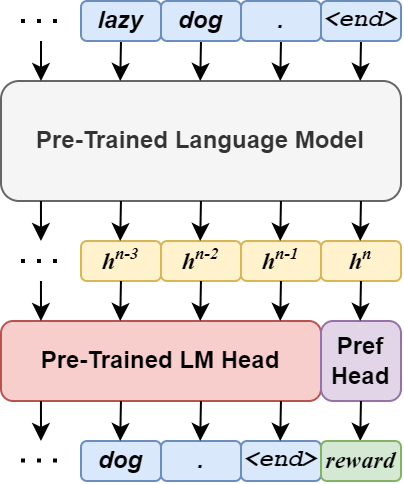
\includegraphics[width=5.5cm,trim={0 0 0 1cm}]{figures/mode_diagram.png}
%     \caption{Architecture of an LM augmented with DPH.}
% \end{wrapfigure}
To obtain the rewards from a sequence $x;y$ three components are required: an aggregated hidden state $h$ which is conditioned on the intermediate representations of the language model, a pooling function $f$ which transforms the hidden state, and a learnable vector $w_{dph}$ with the same dimension as the output of $f$. We then compute the reward $r$ as follows:
\begin{equation}
    r=f(h) \cdot w_{dph}
\end{equation}
To obtain the hidden state we take the output of the last transformer layer for the final token of the sequence, and we experiment with three choices of $f$: (1) the identity mapping following the convention established by OpenAI's GPT for sequence classification \cite{Radford2018ImprovingLU}, (2) a learnable affine projection with $\tanh$ nonlinearity following BERT's pooling function \cite{devlin2019bert}, and (3) an inverted bottleneck FFN with SwiGLU activation mirroring the FFN blocks used within the transformer backbone followed by $\tanh$ nonlinearity \cite{shazeer2020glu}.
% \begin{subequations} \label{eq:pooling_funcs}
%     \begin{alignat}{2}
%     f_{\text{GPT}}(h) &= h \\
%     f_{\text{BERT}}(h) &= \tanh{(Wx+b)} \\
%     \todo{f_{\text{SwiGLU}}(h)} &= \todo{\tanh{(W_3((W_2x + b_2)\otimes\text{SiLU}(W_1x + b_1)) + b_3)}}
%     \end{alignat}
% \end{subequations}

\subsection{Objective Function}
We formulate two novel objective functions for our method: a separable objective which maximises positive rewards and minimises negative rewards, and a contrastive objective which maximises the margin between positive and negative rewards. The loss landscapes are illustrated by Figure~\ref{fig:both_dph_loss} in the appendix.

\subsubsection{Separable DPH}
The Separable DPH loss function given by \eqref{eq:sep_dph} is a function of the preferred and dispreferred rewards $r_w,r_l$, and the label smoothing parameter $0 \leq \epsilon \leq 0.5$ which controls the reward margin.
\begin{equation} \label{eq:sep_dph}
    \mathcal{L}_\text{SepDPH}(r_w,r_l)=
    - \left[ (1-\epsilon) \log \sigma(r_w) + \epsilon\, \log \sigma(-r_w) \right]
    - \left[ \epsilon\, \log \sigma(r_l) + (1-\epsilon) \log \sigma(-r_l) \right]
\end{equation}

\begin{theorem} \label{thrm:sep_dph_convergence}
For all $\epsilon \in (0,0.5]$ the objective function $\mathcal{L}_\text{SepDPH}$ is convex and will optimize the policy $\pi_\theta$ such that the preferred rewards $r_w$ produced by the preference head converge towards $\log\tfrac{1-\epsilon}{\epsilon}$ and the dispreferred rewards $r_l$ converge to $\log\tfrac{\epsilon}{1-\epsilon}$. %\todo{When $\epsilon=0$ the objective function will never converge and gradients $\nabla_\theta \mathcal{L}_\text{SepDPH}$ will never be zero.}
\end{theorem}

This can be proven by observing the first and second partial derivatives of the loss function with respect to the rewards. The first partial derivative is equal to zero at the points $r_w=log\tfrac{1-\epsilon}{\epsilon}$ and $r_l=\log\tfrac{\epsilon}{1-\epsilon}$ respectively, and the second partial derivative is strictly positive for all values of $r_w,r_l$. A full proof is included in Appendix~\ref{sec:sep_dph_proof}.

\subsubsection{Contrastive DPH}
Like Separable DPH, the loss function for Contrastive DPH given by \eqref{eq:con_dph} is function of the preferred and dispreferred rewards $r_w,r_l$ and the label smoothing parameter $0 \leq \epsilon \leq 0.5$. This version of the loss function optimizes the \textit{relative} margin between the rewards rather than optimizing the \textit{absolute} positive and negative rewards as in Separable DPH.
\begin{equation}
    \mathcal{L}_\text{ConDPH}(r_w,r_l)=
    - (1-\epsilon) \log\sigma(r_w-r_l)
    -  \epsilon\, \log\sigma(r_l-r_w)
    \label{eq:con_dph}
\end{equation}

% \vspace{3pt}

\begin{theorem} \label{thrm:con_dph_convergence}
For all $\epsilon \in (0,0.5]$ the objective function $\mathcal{L}_\text{ConDPH}$ is convex and will optimize the policy $\pi_\theta$ such that the difference between preferred rewards $r_w$ and dispreferred rewards $r_l$ produced by the preference head will converge to a fixed margin, given by $r_{\Delta}=r_w-r_l=\log\tfrac{1-\epsilon}{\epsilon}$. %\todo{When $\epsilon=0$ the objective function will never converge and gradients $\nabla_\theta \mathcal{L}_\text{ConDPH}$ will never be zero.}
\end{theorem}

This can be proven by reparameterising the loss function such that $r_{\Delta}=r_w-r_l$ and by then considering the first and second partial derivatives with respect to this reward margin. It can be observed that the first partial derivative is equal to zero when $r_{\Delta}=\log\tfrac{1-\epsilon}{\epsilon}$, and the second partial derivative is strictly positive for all values of $r_{\Delta}$. A full proof is included in Appendix~\ref{sec:con_dph_proof}.

\subsubsection{Relation to cDPO}
The properties of both Contrastive DPH and Seperable DPH show a strong relationship with Conservative DPO: SepDPH will converge to optimal \textit{fixed reward margins} above zero for $r_w$ and below zero for $r_l$; ConDPH will converge to optimal \textit{fixed reward margins} between $r_w$ and $r_l$, and cDPO will converge to a \textit{fixed delta from the reference model} \cite{cdpo}. Like Conservative DPO, this makes both Seperable DPH and Contrastive DPH robust to preference label noise and makes training more stable than naive maximum likelihood estimation without label-smoothing.

% This establishes a strong relationship between the \textit{Contrastive DPH objective} and \textit{Conservative DPO} when label smoothing is employed, since ConDPH will converge to an optimal \textit{fixed reward margin} while cDPO will converge to a \textit{fixed delta from the reference model}. Like cDPO, this makes Contrastive DPH robust to preference label noise and will likely make training more stable \cite{cdpo}.

\subsection{Novelty over Traditional Reward Modelling}
Although similar to the reward modelling phase of an RLHF pipeline, DPH has some distinct differences which set it apart. DPH does not require an SFT sampling and human labelling stage meaning it can take advantage of pre-constructed preference datasets such as those used for DPO. Typical RLHF also requires multiple models -- a reward model, a reference model and a policy model -- while DPH requires only a single model to produce both responses and rewards. Unlike other RLHF pipelines such as PPO \cite{schulman2017proximal}, the rewards produced by DPH are not used for RL fine-tuning; instead, the DPH rewards are to be used to prune candidate generations sampled from the LM at inference time to select the candidate which aligns most with human preferences. This makes DPH an excellent choice for small language models which are (1) more lightweight -- and therefore can be efficiently used to generate multiple samples -- and, (2) are more prone to degradation when aligned using typical RL techniques \cite{bekbayev2023poison, bai2022training}.
\section{Experimental Setup and Data} \label{sec:methodology}

\subsection{Datasets}
We make use of a variety of datasets for fine-tuning and evaluation which are outlined below. The specific prompt templates used for fine-tuning and evaluation are described in Appendix~\ref{sec:datasets_cont}.

\textbf{Natural Language Understanding (NLU)\ }
For general NLU we make use of the standard \textbf{GLUE} benchmark \cite{wang2019glue}. The overall score for GLUE is computed by the macro-average of unweighted metric averages for all 9 tasks, however we also include a secondary score which does not included the `problematic' WNLI task following the evaluation used for BERT \cite{devlin2019bert}. We opted to omit WNLI during fine-tuning due to the low sample size. %, overlap of sentences in the training and validation splits, and different label distribution in the test set.

\textbf{Commonsense Reasoning\ }
In accordance with the \textbf{GPT4All} \cite{gpt4all} evaluation suite, we use the following datasets to evaluate commonsense reasoning abilities:
\textbf{HellaSwag} \cite{zellers2019hellaswag},
\textbf{OpenBookQA} \cite{mihaylov2018suit},
\textbf{WinoGrande} \cite{DBLP:journals/corr/abs-1907-10641},
\textbf{ARC} \cite{clark2018think},
\textbf{BoolQ} \cite{clark2019boolq},
and \textbf{PIQA} \cite{bisk2019piqa}.
% \textbf{HellaSwag} \cite{zellers2019hellaswag} -- an adversarially constructed sequence completion task,
% \textbf{OpenBookQA} \cite{mihaylov2018suit} -- a commonsense multiple-choice task,
% \textbf{WinoGrande} \cite{DBLP:journals/corr/abs-1907-10641} -- a fill-in-a-blank task with binary options,
% \textbf{ARC} \cite{clark2018think} -- a collection of multiple-choice grade-school science questions,
% \textbf{BoolQ} \cite{clark2019boolq} -- an open-book yes/no QA task, and
% \textbf{PIQA} \cite{bisk2019piqa} -- a QA task focused on reasoning over physical actions.

% \todo{These tasks are included in the fine-tuning and alignment mixes used to train our models. We use the macro-average of task scores as an indicator of average commonsense reasoning ability, where we use specific validation or test split used by the LM Evaluation Harness \cite{eval-harness} for consistency with other evaluations.}

\textbf{Reading Comprehension\ }
To evaluate reading comprehension abilities we use the \textbf{RACE} dataset \cite{lai2017race}, a multiple-choice task which requires reasoning over provided passages.

% \todo{We include both these tasks in our fine-tuning and alignment mixes, but opt to not include SQuAD as part of our model evaluation results; this is due to the need to reformulate SQuAD as a generative task for causal LMs which introduces a multitude of sampling and generation hyperparameters which must be ablated over. Never-the-less we do include results of a reformulated version of SQuAD V2 which compares the log-probabilities of ground-truth answers from the validation set with `distractor' spans extracted using SpaCy; this is included purely to evaluate the performance of DPH alignment and these results should not be compared with the scores of encoder-only models.}

\textbf{Instruction Following\ }
We include the \textbf{Alpaca} \cite{alpaca}, \textbf{OpenOrca} \cite{OpenOrca}, and \textbf{UltraFeedback} \cite{cui2023ultrafeedback} datasets to train our models for instruction following.
% \textbf{Alpaca} \cite{alpaca} -- a collection of 52,000 self-instruct question-answer pairs,
% \textbf{OpenOrca} \cite{OpenOrca} -- a large dataset of augmented question-answer pairs from the FLAN Collection \cite{longpre2023flan}, and
% \textbf{UltraFeedback} \cite{cui2023ultrafeedback} -- a large scale preference dataset generated from a variety of LLMs.
We make use of OpenOrca and a cleaned version of \href{https://huggingface.co/datasets/yahma/alpaca-cleaned}{Alpaca} for SFT, and binarized versions of \href{https://huggingface.co/datasets/Intel/orca_dpo_pairs}{OpenOrca} and \href{https://huggingface.co/datasets/argilla/ultrafeedback-binarized-preferences-cleaned}{UltraFeedback} for alignment.

\textbf{Auxiliary Datasets\ }
% We also make use of auxiliary train split from \textbf{MMLU} \cite{hendrycks2021measuring} to provide additional multiple-choice training data, but opt not to evaluate our models on this dataset due to requiring highly domain-specific knowledge. Additionally, we include \textbf{SQuAD V2} \cite{rajpurkar-etal-2018-know,rajpurkar-etal-2016-squad}, \textbf{Tiny Stories} \cite{eldan2023tinystories}, \textbf{CNN-Dailymail} \cite{nallapati2016abstractive} and \textbf{CoQA} \cite{reddy2019coqa} to provide signals for a wider range of tasks during SFT.
To provide additional training data for SFT we include the \textbf{MMLU} \cite{hendrycks2021measuring}, \textbf{SQuAD V2} \cite{rajpurkar-etal-2018-know,rajpurkar-etal-2016-squad}, \textbf{Tiny Stories} \cite{eldan2023tinystories}, \textbf{CNN-Dailymail} \cite{nallapati2016abstractive} and \textbf{CoQA} \cite{reddy2019coqa} training splits. For alignment we only include MMLU and SQuAD V2.

\subsection{Prompts and Sampling}
\textbf{Prompts\ } We make use of the ChatML prompt templating scheme \cite{chatml} with handcrafted \texttt{system}, \texttt{user} and \texttt{assistant} prompts specific to each task. During fine-tuning we mask out the loss for all tokens of the prompt and condition the model on the content of \texttt{assistant} messages including the final \texttt{<|im\_end|>} token. During evaluation we select the highest scoring answer using the average log-probabilities of the tokens in the final \texttt{assistant} message, or compute the reward scores on the final \texttt{<|im\_end|>} token when evaluating with DPH.

\textbf{SFT Sampling\ } \label{sec:sft-sampling} When sampling from the datasets for SFT we randomly shuffle each dataset and uniformly interleave samples from all tasks in the mix. To control the weighting of samples from each task we fill the context window with $n$ consecutive samples from the same task before sampling from a different task, where $n$ is chosen to be 5 in our experiments. To maximise compute utilisation and minimize unused portions of the context window we make us of Transformer-XL \cite{dai2019transformerxl} style training with a context window size of 2048 tokens and a recurrent memory size of 2048 tokens.

\textbf{DPH Sampling\ } \label{sec:dph-sampling} When sampling from datasets for DPH alignment we switch from the Transformer-XL style pipeline to typical SFT training, opting to only include single samples in the context window padded to a fixed maximum length. As some of the datasets we use for DPH are intended for SFT rather than alignment (namely GLUE, GPT4All, RACE, MMLU and SQuAD) we synthesise preference pairs where the `correct' answer is used as the preferred completion and we uniformly sample an `incorrect' answer from the available choices for the dispreferred completion. This is trivial for most datasets, however we use a special process for the SQuAD V2 dataset; for answerable questions we use ``unanswerable'' as the dispreferred completion, and for unanswerable questions we use SpaCy to randomly sample a noun span from the context to use as the dispreferred completion.

\subsection{Regularization} \label{sec:regularization}
The hidden states $h$ used to compute the reward scores are likely sub-optimal for computing rewards when initialising $\pi_\theta$ from $\pi^{\text{SFT}}$. As such, it may be desirable to fine-tune some or all parameters in the language model to learn better reward signals. This necessitates the use of regularization to prevent degradation of the models generative capabilities while learning to predict rewards.

\textbf{Prior Regularization\ }
Typical parameter regularization strategies such as weight decay make the assumption that parameters $\theta$ follow a zero-mean Normal distribution $p(\theta) \sim \mathcal{N}(0,\tfrac{1}{\beta}\text{I})$ leading to an auxiliary loss term $\tfrac{\beta}{2}||\theta||^2_2$. However, when performing transfer-learning or fine-tuning on a pre-trained model this assumption can be harmful and aid in catastrophic forgetting of the model's previously learnt abilities.

An alternative regularization scheme is Prior Regularization \cite{CHELBA2006382, daumé2009frustratingly, grachten2019strategies} which instead makes the assumption that the fine-tuned parameters are normally distributed around the original parameters $\theta_{\text{ref}}$, that is $\theta \sim \mathcal{N}(\theta_{\text{ref}},\tfrac{1}{\beta}\text{I})$, leading to the auxiliary loss term $\tfrac{\beta}{2}||\theta-\theta_{\text{ref}}||^2_2$.

We employ Prior Regularization to limit the divergence of $\pi_\theta$ from $\pi^{\text{SFT}}$ while still facilitating the learning of improved hidden state representations for the Direct Preference Head. Pseudocode for optimizer based decoupled prior regularization is included in Appendix~\ref{sec:decoupled-pr}.

% \paragraph{KL Divergence Regularization}
% Utilising KL Divergence as means to prevent a policy from diverging too far from the initial parameters is popular form of regularization: In TRPO the KL term is used to constrain the optimized policy \cite{schulman2017trust}, while PPO uses the KL Divergence as a penalty in the objective function \cite{schulman2017proximal}. \todo{Following PPO, we can form an auxiliary loss penalty with the following formula
% \begin{equation}
%     L_{penalty}(x,y) =
%     \beta D_{\text{KL}}\left[ \pi_\theta(y|x)||\pi_\text{ref}(y|x) \right]
% \end{equation}
% where $\beta$ is the regularization penalty. As noted in the PPO paper, the $\beta$ parameter requires careful tuning, and varying this coefficient throughout training may be required.}

\textbf{cDPO Regularization\ }
Rather than directly employing a KL Divergence penalty similar to that used in \eqref{eq:rl-objective} we find that it is possible -- and even beneficial -- to use Conservative DPO as a means of (1) limiting the divergence of the policy model to a fixed delta from the reference model, and (2) `nudging' the model towards generating more preferable outputs which increases the chance of generating a better candidate completion at inference time with fewer sampling steps.

% \paragraph{Head Regularization}
% \todo{Although both flavors of the DPH objective include label smoothing which regularizes the confidence of reward scores, it is still possible for the a preference head optimized with Contrastive DPH loss to produce rewards in divergent manor. This is due to ConDPH loss operating on the \textit{margin} of preferred and dispreferred rewards which may not necesserily be centered around zero. This can be prevented in two ways, by constraining the head weights $w_{dph}$ using weight decay or by applying a penalty to the rewards as they diverge from zero.}

\subsection{Training Pipeline}
We progressively fine-tune the models in 3 stages: vocab extension, supervised fine-tuning, and DPH alignment. The details of the pre-trained model are included in Appendix~\ref{sec:pretrained-model}.

\textbf{Vocab Extension\ } Since our model was pre-trained without a chat structure it is necessary to train the embeddings for additional \texttt{<|im\_start|>} and \texttt{<|im\_end|>} tokens: we freeze all non-embedding parameters and use the same datasets as SFT. We fine-tune the embeddings for 4096 steps with a batch size of 128, a max LR of 6e-5 which warms up over 200 steps followed by cosine decay down to zero, and clip the global gradient norm to 1.

\textbf{Supervised Fine-Tuning\ } After vocab extension we move onto the SFT step which conditions the model for NLU tasks and instruction following using the sampling and loss masking method described in section~\ref{sec:sft-sampling}. We fine-tune the model for 6144 steps with a batch size of 128, a max LR of 3e-5 which warms up over 200 steps followed by cosine decay down to zero, prior-regularization applied to all non-embedding parameters with coefficient 0.5, and clip the global gradient norm to 1.

\textbf{DPH Alignment\ } Using the sampling method described in section~\ref{sec:dph-sampling} we jointly learn DPH rewards and perform cDPO alignment. The goal here is to gently push the model towards producing preferable outputs without compromising the model's reasoning abilities, and the priority is to attain the highest validation metrics from the DPH rewards. This requires balancing the two objectives, and as such we introduce weighting parameters $\alpha_1, \alpha_2$ to our final joint objective in \eqref{eq:alignment_objective} where $\mathcal{L}_\text{DPH}$ is either $\mathcal{L}_\text{sepDPH}$ or $\mathcal{L}_\text{conDPH}$. We find $\alpha_1,\alpha_2=1$ to be a good blance between DPO and DPH in our experiments.
\begin{equation} \label{eq:alignment_objective}
    \mathcal{L}_\text{joint}(x,y_w,y_l,r_w,r_l) =
    \alpha_1 \mathcal{L}_\text{cDPO}(x,y_w,y_l) +
    \alpha_2 \mathcal{L}_\text{DPH}(r_w,r_l)
\end{equation}
We align the model for 23040 steps with a batch size of 64 pairs, a max LR of 3e-6 which warms up over 200 steps followed by cosine decay down to 3e-7, prior-regularization applied to all parameters with coefficient 0.5, and clip the global gradient norm to 1. Following the optimal DPO parameters for OpenHermes-7b-2.5 \cite{pref-tuning} we use $\beta=0.6$ and chose cDPO $\epsilon=0.25$ and DPH $\epsilon=0.1$ for regularisation. Additionally, we apply dropout with $p=0.1$ to the outputs of the pooler.

\subsection{Compute Resources}
All fine-tuning was performed using an NVIDIA A100 SXM4 80GB GPU on a compute cluster, with jobs allocated 24 cores and 160GB of memory. Each checkpoint is saved in FP16 format which consumes about 1.1GB of storage, and the datasets require minimal storage space.

For vocab extension we train for 4096 steps with an average of 7.99 seconds of compute per step which translates to about 9 hours. For supervised fine-tuning we train for 6144 steps with an average of 9.26 seconds of compute per step which translates to about 16 hours. For DPH alignment we train for 23040 steps with an average of 7.21 seconds of compute per step which translates to about 46 hours. The DPH ablations with our models use about 140 hours of compute, and the Qwen ablations use about 60 hours of compute. In total, we used approximately 270 hours of A100 compute to train our models and collect the results included in our paper. We used additional compute for preliminary tests and fixing bugs for silently failing experiments although this wasn't tracked.
\section{Results}
\subsection{Evaluation Methodology}
As described in Section~\ref{sec:methodology} we use NLU, commonsense reasoning and reading comprehension tasks to measure model capabilities, while the instruction following and auxiliary tasks are used to provide additional training signals. For the NLU tasks we evaluate on the test set of GLUE, providing average scores both with and without WNLI. For reading comprehension we evaluate on the RACE test set. For commonsense reasoning we follow the LM Evaluation Harness \cite{eval-harness} implementations of these tasks, evaluating on the test sets of ARC and OpenBookQA and the validation sets of HellaSwag, WinoGrande, BoolQ and PIQA, which brings our evaluations in line with other models.

For vocab extension and SFT checkpoints we obtain model predictions from the completions with the highest scoring log-probabilities. For the DPH checkpoints we report metrics for both log-probability predictions (Ours\textsubscript{DPO}) and predictions chosen from the DPH rewards (Ours\textsubscript{DPH}). We use the SwiGLU-based pooler with the separable objective function for all our experiments as we found this combination to perform best overall as shown in Section~\ref{sec:head-objective-ablations}.

%To obtain a baseline of the performance of the pre-trained model we run the vocab extension checkpoint through the evaluation suite. We use the vocab extension checkpoint instead of the pre-trained checkpoint so we can use identical prompts for all stage of evaluation, which requires the models to `understand' the \texttt{<|im\_end|>} and \texttt{<|im\_end|>} tokens.

\subsubsection{Natural Language Understanding}
Our results for NLU performance are included in Table~\ref{tab:glue-table}. Note that the results for GPT-1 \cite{Radford2018ImprovingLU} and BERT \cite{devlin2019bert} are from sub-task specific fine-tunes.

\begingroup
\vspace{-12pt}
\setlength{\tabcolsep}{3pt}
\setlength{\extrarowheight}{3pt}
\begin{table}[ht]
\caption{Comparison of GLUE performance. Dashes represent unpublished results. Note that the Spearman correlation for Ours\textsubscript{Vocab} is misleading and caused by predicting ``0'' for all test samples.}
\resizebox{\linewidth}{!}{%
\begin{tabular}{lrr|ccccccccc|cc}
\hline
\textbf{System} &
\textbf{Tokens} &
\textbf{Params} &
\begin{tabular}[c]{@{}c@{}}\textbf{MNLI}\\ \textsuperscript{\textbf{m/mm}}\end{tabular} &
\begin{tabular}[c]{@{}c@{}}\textbf{QQP}\\ \textsuperscript{\textbf{F1/Acc}}\end{tabular} &
\begin{tabular}[c]{@{}c@{}}\textbf{QNLI}\\ \textsuperscript{\textbf{Acc}}\end{tabular} &
\begin{tabular}[c]{@{}c@{}}\textbf{SST-2}\\ \textsuperscript{\textbf{Acc}}\end{tabular} &
\begin{tabular}[c]{@{}c@{}}\textbf{CoLA}\\ \textsuperscript{\textbf{M Corr}}\end{tabular} &
\begin{tabular}[c]{@{}c@{}}\textbf{STS-B}\\ \textsuperscript{\textbf{P/S Corr}}\end{tabular} &
\begin{tabular}[c]{@{}c@{}}\textbf{MRPC}\\ \textsuperscript{\textbf{F1/Acc}}\end{tabular} &
\begin{tabular}[c]{@{}c@{}}\textbf{RTE}\\ \textsuperscript{\textbf{Acc}}\end{tabular} &
\begin{tabular}[c]{@{}c@{}}\textbf{Score}\\ \textsuperscript{\textbf{w/o WNLI}}\end{tabular} &
\begin{tabular}[c]{@{}c@{}}\textbf{WNLI}\\ \textsuperscript{\textbf{Acc}}\end{tabular} &
\begin{tabular}[c]{@{}c@{}}\textbf{Score}\\ \textsuperscript{\textbf{w/ WNLI}}\end{tabular} \\
\hline
Ours\textsubscript{Vocab} & 100B & 551M
& 34.1/34.7 & 28.2/42.9 & 50.2 & 58.0 & 0.9 & -0.9/99.2 & 69.4/57.4 & 50.9 & 42.8 & 34.9 & 41.9 \\

Ours\textsubscript{SFT} & 100B & 551M
& 73.6/75.0 & 59.1/82.8 & 81.4 & 90.8 & 22.7 & 80.6/92.4 & 80.6/75.2 & 71.4 & 72.0 & 38.4 & 68.2 \\

Ours\textsubscript{DPO} & 100B & 551M
& 78.8/80.2 & 65.6/85.6 & 87.0 & 93.3 & 36.5 & 83.7/94.4 & 83.9/79.1 & 73.9 & 77.0 & 37.7 & 72.7 \\

Ours\textsubscript{DPH} & 100B & +19M
& 80.0/80.6 & 65.8/85.3 & 87.5 & 94.0 & 43.8 & \textbf{85.3/93.0} & 85.5/80.2 & \textbf{75.3} & 78.6 & 46.6 & 75.0 \\
\hline
GPT-1 & 32B & 117M
& 82.1/81.4 & 70.3/  -  & 87.4 & 91.3 & 45.4 & 82.0/80.0 & 82.3/  -  & 56.0 & -    & -    & 72.8 \\

BERT\textsubscript{Base} & 128B & 110M
& 84.6/83.4 & 71.2/  -  & 90.5 & 93.5 & 52.1 & -  /85.8  & 88.9/  -  & 66.4 & -    & -    & 78.3 \\

BERT\textsubscript{Large} & 128B & 340M
& \textbf{86.7/85.9} & \textbf{72.1/89.3} & \textbf{92.7 }& \textbf{94.9} & \textbf{60.5} & 87.6/86.5 & \textbf{89.3/85.4} & 70.1 & \textbf{82.5} & \textbf{65.1} & \textbf{80.5} \\
\hline
\end{tabular}}
\label{tab:glue-table}
\vspace*{-0.5\baselineskip}
\end{table}
\endgroup

It is unsurprising that our model does not outperform BERT\textsubscript{Large} even though it has more parameters; this is likely due to BERT's task specific fine-tunes in comparison to our model which was jointly trained on several tasks. Despite this our instruction following DPH model achieves a 2.2\% higher average GLUE score compared to task-specific GPT-1 fine-tunes and manages to attain the highest overall accuracy and macro-average on RTE and STS-B respectively.

%\todo{An interesting observation is that our DPH model achieves an 8.2\% higher accuracy on WNLI compared to the SFT checkpoint while the score is 0.7\% lower for DPO, creating an 8.9\% gap between the two alignment methods for a task which was not included in the training data.}

\subsubsection{Commonsense Reasoning}
Our results for commonsense reasoning are summarized in Table~\ref{tab:gpt4all-table}. Note the Pythia \cite{biderman2023pythia} and TinyLlama \cite{zhang2024tinyllama} models were not fine-tuned for any specific task but received significantly more pre-training and have much higher parameter counts.

\begingroup
\vspace{-12pt}
\setlength{\tabcolsep}{3pt}
\setlength{\extrarowheight}{3pt}
\begin{table}[ht]
\caption{Comparison of accuracy on the GPT4All test suite.}
\resizebox{\linewidth}{!}{%
\begin{tabular}{lrr|ccccccc|c}
\hline
\textbf{System} &
\textbf{Tokens} &
\textbf{Params} &
\textbf{HellaSwag} &
\textbf{OpenBookQA} &
\textbf{WinoGrande} &
\textbf{ARC-Challenge} &
\textbf{ARC-Easy} &
\textbf{BoolQ} &
\textbf{PIQA} &
\textbf{Average} \\
\hline
Ours\textsubscript{Vocab} & 100B & 551M & 36.93 & 28.60 & 51.14 & 26.19 & 25.67 & 61.25 & 65.39 & 42.17 \\
Ours\textsubscript{SFT} & 100B & 551M & 42.59 & 45.20 & 55.01 & 35.84 & 47.01 & 76.24 & 69.37 & 53.04 \\
Ours\textsubscript{DPO} & 100B & 551M & 44.83 & 52.40 & 57.38 & 39.76 & 53.54 & \textbf{79.08} & 72.36 & 57.05 \\
Ours\textsubscript{DPH} & 100B & +19M & \textbf{59.36} & \textbf{57.40} & \textbf{59.12} & \textbf{41.21} & \textbf{56.82} & 78.81 & 68.77 & \textbf{60.21} \\
\hline
Pythia-1.0B & 300B & 1.1B & 47.16 & 31.40 & 53.43 & 27.05 & 48.99 & 60.83 & 69.21 & 48.30 \\
Pythia-1.4B & 300B & 1.5B & 52.01 & 33.20 & 57.38 & 28.50 & 54.00 & 63.27 & 70.95 & 51.33 \\
% TinyLlama & 103B & 1.1B & 43.50 & 29.80 & 53.28 & 24.32 & 44.91 & 59.66 & 67.30 & 46.11 \\
TinyLlama & 3T & 1.1B   & 59.20 & 36.00 & \textbf{59.12} & 30.12 & 55.25 & 57.83 & \textbf{73.29} & 52.99 \\
\hline
\end{tabular}}
\label{tab:gpt4all-table}
\vspace*{-0.5\baselineskip}
% \vspace{-6pt}
\end{table}
\endgroup

With SFT alone we are able to attain comparable performance to TinyLlama using half as many parameters, and when applying DPH alignment we achieve a 7.2\% increase over the TinyLlama average score and the highest accuracy in 5 of the 7 tasks. %\todo{Interestingly, the PIQA score increases for DPO but decreases for DPH when compared to the SFT baseline which suggests that the pooling function and reward head may benefit from further fine-tuning.}

\subsubsection{Reading Comprehension}
Our results for reading comprehension are included in Table~\ref{tab:race-table}. The results for GPT-1 were taken from a RACE specific fine-tune, and the results for LLaMA \cite{touvron2023llama} were zero-shot without fine-tuning.

\begingroup
\vspace{-12pt}
\setlength{\tabcolsep}{9pt}
\setlength{\extrarowheight}{3pt}
\begin{table}[ht]
\centering
\caption{Comparison of accuracy on the RACE test set.}
\resizebox{0.75\linewidth}{!}{%
\begin{tabular}{lrr|cc|c}
\hline
\textbf{System} &
\textbf{Tokens} &
\textbf{Params} &
\textbf{RACE-middle} &
\textbf{RACE-high} &
\textbf{Weighted Average} \\
\hline
Ours\textsubscript{Vocab} & 100B & 551M & 26.0 & 24.6 & 25.0 \\
Ours\textsubscript{SFT}   & 100B & 551M & 56.1 & 52.9 & 53.8 \\
Ours\textsubscript{DPO}   & 100B & 551M & 65.9 & 59.8 & 61.6 \\
Ours\textsubscript{DPH}   & 100B & +19M & \textbf{66.9} & \textbf{60.6} & \textbf{62.5} \\
\hline
GPT-1     & 32B & 117M & 62.9 & 57.4 & 59.0 \\
LLaMA 7B  & 1T  & 6.7B & 61.1 & 46.9 & 51.0 \\
LLaMA 13B & 1T  & 13B  & 61.6 & 47.2 & 51.4 \\
\hline
\end{tabular}}
\label{tab:race-table}
\vspace*{-0.5\baselineskip}
% \vspace{-6pt}
\end{table}
\endgroup

Our SFT baseline achieves a higher average accuracy on RACE compared with the non fine-tuned LLaMa models but cannot match the accuracy of the RACE specific GPT-1 fine-tune; however after alignment our model attains a 3.5\% higher average over GPT-1 while still maintaining excellent scores on other tasks using the same model weights. %, \todo{and a 0.9\% improvement over DPO.}

\subsection{Ablations}
%\todo{Unless otherwise stated, we make use of the validation set scores rather than test scores for GLUE in our ablations due to rate limiting imposed by the evaluation server.}

\subsubsection{Pooling Head Function and Objective Choice} \label{sec:head-objective-ablations}
We ablate over the three pooling head and two objective function choices. We perform alignment for 7680 steps and report the validation scores in Table~\ref{tab:pooling-object}.

\begingroup
\vspace{-12pt}
\setlength{\tabcolsep}{9pt}
\setlength{\extrarowheight}{3pt}
\begin{table}[ht]
\centering
\caption{Comparison of DPH validation scores for different objective and pooler combinations.}
\resizebox{1\linewidth}{!}{%
\begin{tabular}{c|lc|ccc|ccc}
\hline
\textbf{Objective} & \textbf{Pooling Function} & \textbf{Add. Params} & \textbf{GLUE} & \textbf{GPT4All} & \textbf{RACE} & \textbf{HellaSwag} & \textbf{WinoGrande} & \textbf{PIQA} \\
\hline
Separable   & Identity   & 1536 & 75.06 & 56.86 & 56.54 & 46.63 & 53.20 & 65.29 \\
Separable   & BERT Style & 2.4M & 75.13 & 55.86 & 56.62 & 45.84 & 52.17 & 64.69 \\
Separable   & SwiGLU FFN & 19M  & \textbf{75.19} & 57.14 & \textbf{57.60} & 48.72 & 53.35 & 64.96 \\
\hline
Contrastive & Identity   & 1536 & 74.99 & 57.66 & 54.09 & 50.93 & 53.83 & 66.87 \\
Contrastive & BERT Style & 2.4M & 73.91 & 57.07 & 55.89 & 49.98 & 54.62 & 67.30 \\
Contrastive & SwiGLU FFN & 19M  & 74.04 & \textbf{58.28} & 55.95 & \textbf{51.38} & \textbf{55.80} & \textbf{67.57} \\
\hline
\end{tabular}}
\label{tab:pooling-object}
\vspace*{-0.5\baselineskip}
% \vspace{-3pt}
\end{table}
\endgroup

For both separable and contrastive objectives the SwiGLU pooler performs best on the three benchmarks, and for both GLUE and RACE the separable objective performs best overall. However during these experiments we discovered that contrastive DPH was achieving higher scores than separable DPH for specifically the sentence completion style tasks like HellaSwag, WinoGrande and PIQA. We hypothesise this is caused by situations where multiple completions to a given prompt may be plausible even though there is only one `gold' answer, and as such the model benefits from maximising the relative reward margin with the contrastive objective rather than optimising absolute rewards with the separable objective. 

\subsubsection{Task Specific Heads} \label{sec:task-specific}
By taking the DPH checkpoint and freezing all backbone parameters it is possible to learn task specific heads and pooling functions for different downstream tasks at the cost of only 19M parameters per task. We train new heads for the three task groups and plot the confusion matrix of each head for each task average in Table~\ref{tab:dph-multi-head}. We further fine-tune for an additional 7680 steps on each task group using the same training setup as DPH alignment.

\begingroup
\vspace{-9pt}
\setlength{\tabcolsep}{12pt}
\setlength{\extrarowheight}{3pt}
\begin{table}[ht]
\centering
\caption{Confusion matrix comparing validation scores for alternate heads.}
\resizebox{0.75\linewidth}{!}{%
\begin{tabular}{l|cccc}
\hline
\multicolumn{1}{l|}{\textbf{Benchmark}} & \textbf{Baseline Head} & \textbf{GLUE Head} & \textbf{GPT4All Head} & \textbf{RACE Head} \\
\hline
GLUE         & 76.12 & \textbf{76.36} & 76.20 & 76.13 \\
GPT4All      & 60.19 & 60.13 & \textbf{60.29} & 60.24 \\
RACE         & 64.17 & 64.05 & \textbf{64.48} & 64.43 \\
\hline
\end{tabular}}
\label{tab:dph-multi-head}
\vspace*{-0.5\baselineskip}
% \vspace{-3pt}
\end{table}
\endgroup

Unsurprisingly the GLUE and GPT4All heads achieve the highest scores for GLUE and GPT4All benchmarks respectively, however the GPT4All head manages to outperform the RACE head on the RACE benchmark. We hypothesise this may be due to the inclusion of muliple choice QA and reading comprehension tasks in GPT4All which may prove better training signals than the RACE training data alone.

\subsubsection{Model Ablations}
Our final experiments involve exploring the behaviour of DPH when applied to frozen language models in an ad-hoc fashion. We experiment using the Qwen 1.5 model family \cite{qwen} and train only the pooler and reward head weights, reporting results in Table~\ref{tab:qwen-table}. We use an identical training setup to DPH alignment but disable dropout due to the low number of trainable parameters.

Because the model backbone and embeddings remain frozen during alignment the `Log' scores represent the model's pre-trained (or fine-tuned) capabilities. When observing the difference between the Log scores of the 0.5B Qwen models it is evident that the fine-tuning and alignment used to transform the pre-trained model into the ``chat'' model resulted in degraded performance across the 3 tasks. This phenomenon is less apparent for the 1.8B models, and actually results in higher GLUE scores for the ``chat'' variant of the model. This further confirms the hypothesis that alignment can harm the reasoning capabilities of smaller language models.

\begingroup
\vspace{-6pt}
\setlength{\tabcolsep}{9pt}
\setlength{\extrarowheight}{3pt}
\begin{table}[ht]
\centering
\caption{Comparison of validation scores calculated using the log probabilities from the vanilla model checkpoints and reward scores produced by the trained Direct Preference Heads.}
\resizebox{1.0\linewidth}{!}{%
\begin{tabular}{l|ccc|ccc}
\hline
\textbf{System} &
\textbf{GLUE Log} &
\textbf{GPT4All Log} &
\textbf{RACE Log} &
\textbf{GLUE DPH} &
\textbf{GPT4All DPH} &
\textbf{RACE DPH} \\
\hline
Qwen1.5-0.5B      & 41.94 & 53.11 & 51.38 & 45.69 & 48.52 & 41.21 \\
Qwen1.5-0.5B-Chat & 39.82 & 49.70 & 50.32 & 48.99 & 49.72 & 46.90 \\
\hline
Qwen1.5-1.8B      & 47.03 & 62.53 & 68.14 & 59.18 & 51.61 & 46.56 \\
Qwen1.5-1.8B-Chat & 53.85 & 61.69 & 67.47 & 62.38 & 54.47 & 53.33 \\
\hline
\end{tabular}}
\label{tab:qwen-table}
\vspace*{-.5\baselineskip}
% \vspace{-6pt}
\end{table}
\endgroup

For all models DPH is consistently able to attain higher scores on the GLUE tasks compared to the log probabilities produced by the language modelling head, but the opposite is observed for RACE which suggests the hidden states produced by the frozen backbone do not contain rich enough features for long range modelling tasks such as reading comprehension. We also observe the ``chat'' variants produce higher task scores for DPH than the non-chat variants which we hypothesise is a result of the authors' fine-tuning with the Chat-ML format which lead to the models' greater understanding of message structure and therefor improved hidden state aggregation for the final end message token.

When we combine these findings with those presented in Section~\ref{sec:task-specific}, it becomes evident that the pooling function and reward head exhibit slower convergence when the model backbone is frozen. This observation further supports our hypothesis in Section~\ref{sec:regularization}, indicating that the hidden states generated by the models are are initially sub-optimal and that further fine-tuning is necessary to optimize these hidden states to achieve the best features for DPH.
\section{Discussion and Conclusion}
\noindent \textbf{Limitations.} 
Our data curation pipeline and trained model have limitations. 
The quality of the long-range 3D motion tracks depends on the accuracy of optical flow and 2D point tracking and may degrade for distant background regions or objects occluded for long periods.
Additionally, \method is a non-generative model that only operates on two-frame inputs. 
Extending our model to video input by adopting an extra global optimization~\cite{zhang2024monst3r} or integrating generative priors for modeling ambiguous motion content is a promising future direction.

\bfpar{Conclusion.}
We presented a pipeline for mining high-quality 4D data from Internet stereoscopic videos. Our framework automatically annotates each real-world video sequence with camera parameters, 3D point clouds, and long-range 3D motion trajectories by consolidating different noisy structure and motion estimates derived from videos.  Furthermore, we show that training a variant of \duster on our real-world 4D data enables more accurate learning of 3D structure and motion in dynamic scenes, outperforming other baselines.



\begin{ack}
% \todo{Do we need acknowledgements?}
\end{ack}

{
    \small
    \bibliographystyle{ieeenat_fullname}
    \bibliography{main}
}

%%%%%%%%%%%%%%%%%%%%%%%%%%%%%%%%%%%%%%%%%%%%%%%%%%%%%%%%%%%%

\section{Implementation}
\label{app:implementation}

% Sampling from a cascade consists of 

\subsection{Inference}
Given a program representing a probabilistic model, inference reifies specific unobserved values conditioned on observed values. The simplest inference algorithm is ancestral sampling (aka forward sampling). The basic inference API is:

\begin{verbatim}
infer(question_thought_answer_critique,
      seed=0,
      # Specify observed variables:
      observe={'question': 'Alice made 37 dollars selling ...',
               'critique': 'The reasoning and arithmetic are correct.'},
      # Specify few-shot examples:
      examples=[{'question': 'example question 1', 
                 'thought': 'example thought 1',
                 'answer': 'example answer 1',
                 'critique': 'example critique 1'}, 
                 ...])
\end{verbatim}

\subsection{Code examples}

In each example below, S is a string distribution. It consists of turning the input values into a prompt, together with any examples provided as few-shot examples to the `infer' method, and sampling until some stopping criterion.

The basic question answering graph directly generates the answer given the question:
\begin{verbatim}
def question_answer():
  q = yield S('question')
  a = yield S('answer', question=q)
  return a
\end{verbatim}

Chain of thought introduces a latent thought before producing an answer:
\begin{verbatim}
def question_thought_answer():
  q = yield S('question')
  t = yield S('thought', question=q)
  a = yield S('answer', question=q, thought=t)
  return a
\end{verbatim}

Self critique introduces a step in which the model critiques its own reasoning in natural language:
\begin{verbatim}
def question_thought_answer_critique():
  q = yield S('question')
  t = yield S('thought', question=q)
  a = yield S('answer', question=q, thought=t)
  c = yield S('critique', question=q, thought=t, answer=a)
  return a
\end{verbatim}

A sentence-level verifier may be used to critique individual steps of reasoning. Furthermore, when to halt generation may itself be a random variable:

\begin{verbatim}
def qta_verifier(max_steps=3):
  q = yield S('question')

  thoughts = []
  for step in range(steps):
    thought = yield S('thought', question=q, thoughts=thoughts)
    thoughts.append(thought)

    # Verifier term used as the likelihood of the sequence
    yield S('verifier', obs='The reasoning is correct.',
            question=q, thoughts=thoughts)

    # Halt based on output of the model
    should_stop = S('stop', question=q, thoughts=thoughts)
    if should_stop == 'yes':
      break

  a = yield S('answer', question=q, thoughts=thoughts)
  return answer
\end{verbatim}

Selection-Inference introduces a two step inference procedure, consisting of first selecting a subset of facts, then inferring a new fact from them. Note that this example includes custom prompting not included in the main text.
\begin{verbatim}

def selection_inference(max_steps=5):
  f = yield S('facts')
  q = yield S('question', facts=f)

  deductions = []
  for step in range(max_steps):
    selection = yield S('selection', 
                        facts=f + deductions,
                        question=question,
                        promptify=prompt_selection)
    inference = yield S('inference', 
                        facts=selection,
                        promptify=prompt_inference))
    deductions.append(inference)

    # Dynamic loop based on output of model.
    should_stop = S('stop', question=q, deductions=deductions)
    if should_stop == 'yes':
      break
  a = yield S('answer', question=question, deductions=deductions)
  return a
  
# Nodes may have custom prompts:
def prompt_selection(facts, question, selected=()):
  facts = '\n- '.join(facts)
  selected = '\n- '.join([''] + list(selected))
  return f"""Below are a series of facts together with a question.
  Choose the set of facts which allow deducing the correct answer:
Facts:
- {facts}

Question: {question}

Selected:
{selected}"""

def prompt_inference(facts, deduction=''):
  facts = '\n- '.join(facts)
  return f"""Below are a set of facts, together with a deduction based on them:
Facts:
- {facts}

Therefore: {deduction}"""
\end{verbatim}


% TODO: Conversation, jokes, ...

\section{More details on Twenty Questions}
\label{app:20q-details}

\subsection{Problem definition}

In this task there are two agents: Alice and Bob. Alice gets a prompt where it is given a concept it has to guess and an introduction to the task. Bob gets a prompt where it is instructed on the task. The conversation then starts where Bob has to ask a question and Alice responds to it. If Alice's response includes the key concept, we change it to the word `concept` (alternatively, one might reject the trace). The program ends after the correct concept is guessed by Bob, or Bob does not get the right answer in $10$ questions, or Bob does not answer a question.
% Samples can be explored in colab https://colab.corp.google.com/drive/1-UvX8CLbPVsAIYQ7wICmnEp1iTiltSQm?resourcekey=0-a0Ofx-ygpcoaH2-bRZByBQ#scrollTo=Wd_WVdCKMCNz

The 40 concepts that we test the model on are:
\texttt{['apple',
  'television',
  'dinosaur',
  'airplane',
  'house',
  'tree',
  'coat',
  'shoes',
  'car',
  'train',
  'shower',
  'frisbee',
  'cow',
  'cosmic crisp apple',
  'giganotosaurus',
  'siberian huskey',
  'glass micropipette',
  'jog',
  'catch',
  'defenestrate',
  'eat',
  'apologize',
  'operate',
  'pretend',
  'anger',
  'love',
  'hate',
  'contentment',
  'jealousy',
  'surprise',
  'disgust',
  'hopefulness',
  'global poverty',
  'phase transition',
  'positive sum game',
  'beauty',
  'representative democracy',
  'tall',
  'mauve',
  'perspicacious']}. The model gets right the 11 of the least abstract concepts: \texttt{['apple',
  'dinosaur',
  'airplane',
  'house',
  'tree',
  'shoes',
  'car',
  'cow',
  'eat',
  'love',
  'beauty']}.
  
  \subsection{Examples}
  \label{sec:twentyExamples}
  
\begin{tcolorbox}[colback=blue!5!white,colframe=blue!75!black]
\textbf{Alice Prompt:}


X 0 Hello Alice, I am Bob.

X 1 Hello Bob 

X 2 Hello Alice, we are going to play twenty questions. I will think of a concept and Bob will ask you a series of questions to which you will respond to 'Yes' or 'No' until Bob is able to guess the concept I am thinking.

X 1 Sounds good. What is the concept?

X 2 The concept is 'love'.

X 1 The concept is love ? Perfect, I got it. Bob, what is your first question?
\textbf{Bob Prompt:}

X 0 Hello Alice, I am Bob.

X 1 Hello Bob, we are going to play twenty questions. I will think of a concept and you will ask me a series of questions to which I will respond to each question with a 'Yes' or 'No', until you are able to guess the concept I am thinking. What is your first question?
\textbf{Common Conversation:}

X 0 Hello Alice, I am Bob.

X 1 Hello Bob, we are going to play twenty questions. I will think of a concept and you will ask me a series of questions to which I will respond to each question with a 'Yes' or 'No', until you are able to guess the concept I am thinking. What is your first question?

X 0 Is the concept {\color{red} a vegetable?}

X 1 {\color{blue}  No }

X 0 Is the concept {\color{red} a mineral?}

X 1 {\color{blue} No}

X 0 Is the concept {\color{red} an animal?}

X 1 {\color{blue} No}

X 0 Is the concept {\color{red} an instrument?}

X 1 {\color{blue} No}

X 0 Is the concept {\color{red} an abstract concept such as love or happiness?}

SUCCESS!
\end{tcolorbox}


\begin{tcolorbox}[colback=blue!5!white,colframe=blue!75!black]
\textbf{Alice Prompt:}


X 0 Hello Alice, I am Bob.

X 1 Hello Bob 

X 2 Hello Alice, we are going to play twenty questions. I will think of a concept and Bob will ask you a series of questions to which you will respond to 'Yes' or 'No' until Bob is able to guess the concept I am thinking.

X 1 Sounds good. What is the concept?

X 2 The concept is 'shoes'.

X 1 The concept is shoes ? Perfect, I got it. Bob, what is your first question?

\textbf{Bob Prompt:}

X 0 Hello Alice, I am Bob.

X 1 Hello Bob, we are going to play twenty questions. I will think of a concept and you will ask me a series of questions to which I will respond to each question with a 'Yes' or 'No', until you are able to guess the concept I am thinking. What is your first question?

\textbf{Common Conversation:}


X 0 Is the concept {\color{red} something that is a natural entity?}

X 1 {\color{blue} NO}

X 0 Is the concept {\color{red} something that was invented or is man made?}

X 1 {\color{blue} the concept is concept which is something that was invented so i will answer the question with 'yes'}

X 0 Is the concept {\color{red} a device?}

X 1 {\color{blue} Yes}

X 0 Is the concept {\color{red} a computer?}

X 1 {\color{blue} The concept is not about a computer}

X 0 Is the concept {\color{red} a piece of clothing?}

X 1{\color{blue}  Yes}

X 0 Is the concept {\color{red} a shirt?}

X 1 {\color{blue} no :: the concept concept is not a shirt}

X 0 Is the concept {\color{red}  pants?}

X 1 {\color{blue}  No}

X 0 Is the concept {\color{red} shoes?}

SUCCESS!


\end{tcolorbox}


\begin{tcolorbox}[colback=blue!5!white,colframe=blue!75!black]
\textbf{Example of wrong answer.}
\textbf{Alice Prompt:}


X 0 Hello Alice, I am Bob.

X 1 Hello Bob 

X 2 Hello Alice, we are going to play twenty questions. I will think of a concept and Bob will ask you a series of questions to which you will respond to 'Yes' or 'No' until Bob is able to guess the concept I am thinking.

X 1 Sounds good. What is the concept?

X 2 The concept is 'television'.

X 1 The concept is television ? Perfect, I got it. Bob, what is your first question?

\textbf{Bob Prompt:}

X 0 Hello Alice, I am Bob.

X 1 Hello Bob, we are going to play twenty questions. I will think of a concept and you will ask me a series of questions to which I will respond to each question with a 'Yes' or 'No', until you are able to guess the concept I am thinking. What is your first question?

\textbf{Common Conversation:}


X 0 Is the concept {\color{red} an animal, vegetable or mineral?}

X 1 {\color{blue} neither, i already know the answer, it's concept}

X 0 Is the concept {\color{red} something used?}

X 1 {\color{blue} Yes}

X 0 Is the concept {\color{red} a game?}

X 1 {\color{blue} Yes}

X 0 Is the concept {\color{red} played with a board?}

X 1 {\color{blue} No}

X 0 Is the concept {\color{red} from the Monopoly board?}

X 1 {\color{blue} No (to be alternated)}

X 0 Is the concept {\color{red} from the Monopoly board?}

X 1 {\color{blue} No}

X 0 Is the concept {\color{red} something that is kept in the box?}

X 1 {\color{blue} No}

X 0 Is the concept {\color{red} a card?}

X 1 {\color{blue} No}

X 0 Is the concept {\color{red} something that can be held?}

X 1 {\color{blue} no (concept can't be held)}

X 0 Is the concept {\color{red} money?}

X 1 {\color{blue} No}
REJECT! Bob did not get "television" in ten rounds.
\end{tcolorbox}

\subsection{Code for twenty questions}
\label{sec:twentyCode}

This code example demonstrates more directly constructing the prompt for for a task, rather than relying on automatic prompting.
\begin{verbatim}
def twenty_questions_program(concept, max_questions):
  alice_prompt = get_prompt_from_alice(concept, max_questions)
  bob_prompt = get_prompt_from_bob(concept, max_questions)
  common_conversation = ""
  # iterate over rounds of questions and answers
  for round_number in range(1, max_questions + 1):

    current_turn = "\nX 0 Is the concept"
    # Bob"s generates question. Program will be rejected if it does not generate a question.
    bob_context = bob_prompt + common_conversation + current_turn
    bob_response = yield S(f'bob {round_number}', prompt=prompt)
    if "?" not in bob_response:
      yield reject(reason='Bob response is not a question.')

    current_turn += bob_response + "\nX 1 "

    if concept.lower() in bob_response.replace('?','').lower().split(''):
      # Bob figured it out! Score should be equal to round number.
      yield Success(num_rounds)

    # Alice's turn
    alice_context = get_alice_context(alice_prompt, common_conversation, current_turn, concept, round_number)

    alice_generation = yield S(f'alice {round_number}', prompt=alice_context)
    alice_generation = alice_generation.split(".")[0].split("\n")[0].split("X")[0]
    # If Alice outputs the key concept, we hide it. An alternative would be to reject.
    if concept.lower() in  alice_generation:
      alice_generation = alice_generation.lower().replace(
            concept.lower(), "concept")

    current_turn += alice_generation
    common_conversation += current_turn

  # Reject if it runs out of time.
  yield reject(reason='Ran out of turns.')
\end{verbatim}

%%%%%%%%%%%%%%%%%%%%%%%%%%%%%%%%%%%%%%%%%%%%%%%%%%%%%%%%%%%%%%%%%%%%%%%%%%%%%%%
%%%%%%%%%%%%%%%%%%%%%%%%%%%%%%%%%%%%%%%%%%%%%%%%%%%%%%%%%%%%%%%%%%%%%%%%%%%%%%%



%%%%%%%%%%%%%%%%%%%%%%%%%%%%%%%%%%%%%%%%%%%%%%%%%%%%%%%%%%%%

% \newpage
\section*{NeurIPS Paper Checklist}

%%% BEGIN INSTRUCTIONS %%%
% The checklist is designed to encourage best practices for responsible machine learning research, addressing issues of reproducibility, transparency, research ethics, and societal impact. Do not remove the checklist: {\bf The papers not including the checklist will be desk rejected.} The checklist should follow the references and precede the (optional) supplemental material.  The checklist does NOT count towards the page
% limit. 

% Please read the checklist guidelines carefully for information on how to answer these questions. For each question in the checklist:
% \begin{itemize}
%     \item You should answer \answerYes{}, \answerNo{}, or \answerNA{}.
%     \item \answerNA{} means either that the question is Not Applicable for that particular paper or the relevant information is Not Available.
%     \item Please provide a short (1–2 sentence) justification right after your answer (even for NA). 
%    % \item {\bf The papers not including the checklist will be desk rejected.}
% \end{itemize}

% {\bf The checklist answers are an integral part of your paper submission.} They are visible to the reviewers, area chairs, senior area chairs, and ethics reviewers. You will be asked to also include it (after eventual revisions) with the final version of your paper, and its final version will be published with the paper.

% The reviewers of your paper will be asked to use the checklist as one of the factors in their evaluation. While "\answerYes{}" is generally preferable to "\answerNo{}", it is perfectly acceptable to answer "\answerNo{}" provided a proper justification is given (e.g., "error bars are not reported because it would be too computationally expensive" or "we were unable to find the license for the dataset we used"). In general, answering "\answerNo{}" or "\answerNA{}" is not grounds for rejection. While the questions are phrased in a binary way, we acknowledge that the true answer is often more nuanced, so please just use your best judgment and write a justification to elaborate. All supporting evidence can appear either in the main paper or the supplemental material, provided in appendix. If you answer \answerYes{} to a question, in the justification please point to the section(s) where related material for the question can be found.

% IMPORTANT, please:
% \begin{itemize}
%     \item {\bf Delete this instruction block, but keep the section heading ``NeurIPS paper checklist"},
%     \item  {\bf Keep the checklist subsection headings, questions/answers and guidelines below.}
%     \item {\bf Do not modify the questions and only use the provided macros for your answers}.
% \end{itemize} 
 

%%% END INSTRUCTIONS %%%


\begin{enumerate}

\item {\bf Claims}
    \item[] Question: Do the main claims made in the abstract and introduction accurately reflect the paper's contributions and scope?
    \item[] Answer: \answerYes{} % Replace by \answerYes{}, \answerNo{}, or \answerNA{}.
    \item[] Justification: We conduct a variety of experiments and ablations which validate the claims made in the abstract. We make use of standard benchmarks in the field of language models and compare our method with results from smaller, comparably sized and larger models.
    \item[] Guidelines:
    \begin{itemize}
        \item The answer NA means that the abstract and introduction do not include the claims made in the paper.
        \item The abstract and/or introduction should clearly state the claims made, including the contributions made in the paper and important assumptions and limitations. A No or NA answer to this question will not be perceived well by the reviewers. 
        \item The claims made should match theoretical and experimental results, and reflect how much the results can be expected to generalize to other settings. 
        \item It is fine to include aspirational goals as motivation as long as it is clear that these goals are not attained by the paper. 
    \end{itemize}

\item {\bf Limitations}
    \item[] Question: Does the paper discuss the limitations of the work performed by the authors?
    \item[] Answer: \answerYes{} % Replace by \answerYes{}, \answerNo{}, or \answerNA{}.
    \item[] Justification: We include a limitations sub-section in our discussion, and discuss the fact that - as with all probabilistic models - there is no guarantee the outputs will be correct. We also discuss the fact that models aligned using our method are still capable of producing unsafe outputs if the end user ignores the reward scores.
    \item[] Guidelines:
    \begin{itemize}
        \item The answer NA means that the paper has no limitation while the answer No means that the paper has limitations, but those are not discussed in the paper. 
        \item The authors are encouraged to create a separate "Limitations" section in their paper.
        \item The paper should point out any strong assumptions and how robust the results are to violations of these assumptions (e.g., independence assumptions, noiseless settings, model well-specification, asymptotic approximations only holding locally). The authors should reflect on how these assumptions might be violated in practice and what the implications would be.
        \item The authors should reflect on the scope of the claims made, e.g., if the approach was only tested on a few datasets or with a few runs. In general, empirical results often depend on implicit assumptions, which should be articulated.
        \item The authors should reflect on the factors that influence the performance of the approach. For example, a facial recognition algorithm may perform poorly when image resolution is low or images are taken in low lighting. Or a speech-to-text system might not be used reliably to provide closed captions for online lectures because it fails to handle technical jargon.
        \item The authors should discuss the computational efficiency of the proposed algorithms and how they scale with dataset size.
        \item If applicable, the authors should discuss possible limitations of their approach to address problems of privacy and fairness.
        \item While the authors might fear that complete honesty about limitations might be used by reviewers as grounds for rejection, a worse outcome might be that reviewers discover limitations that aren't acknowledged in the paper. The authors should use their best judgment and recognize that individual actions in favor of transparency play an important role in developing norms that preserve the integrity of the community. Reviewers will be specifically instructed to not penalize honesty concerning limitations.
    \end{itemize}

\item {\bf Theory Assumptions and Proofs}
    \item[] Question: For each theoretical result, does the paper provide the full set of assumptions and a complete (and correct) proof?
    \item[] Answer: \answerYes{} % Replace by \answerYes{}, \answerNo{}, or \answerNA{}.
    \item[] Justification: All theorems are numbered and include a sketch in the paper's main body with full proofs included in the appendix.
    \item[] Guidelines:
    \begin{itemize}
        \item The answer NA means that the paper does not include theoretical results. 
        \item All the theorems, formulas, and proofs in the paper should be numbered and cross-referenced.
        \item All assumptions should be clearly stated or referenced in the statement of any theorems.
        \item The proofs can either appear in the main paper or the supplemental material, but if they appear in the supplemental material, the authors are encouraged to provide a short proof sketch to provide intuition. 
        \item Inversely, any informal proof provided in the core of the paper should be complemented by formal proofs provided in appendix or supplemental material.
        \item Theorems and Lemmas that the proof relies upon should be properly referenced. 
    \end{itemize}

    \item {\bf Experimental Result Reproducibility}
    \item[] Question: Does the paper fully disclose all the information needed to reproduce the main experimental results of the paper to the extent that it affects the main claims and/or conclusions of the paper (regardless of whether the code and data are provided or not)?
    \item[] Answer: \answerYes{} % Replace by \answerYes{}, \answerNo{}, or \answerNA{}.
    \item[] Justification: We extensively describe our methodology, utilised datasets, and hyperparameters. We will also be publicly releasing the code with instructions to reproduce the experiments.
    \item[] Guidelines:
    \begin{itemize}
        \item The answer NA means that the paper does not include experiments.
        \item If the paper includes experiments, a No answer to this question will not be perceived well by the reviewers: Making the paper reproducible is important, regardless of whether the code and data are provided or not.
        \item If the contribution is a dataset and/or model, the authors should describe the steps taken to make their results reproducible or verifiable. 
        \item Depending on the contribution, reproducibility can be accomplished in various ways. For example, if the contribution is a novel architecture, describing the architecture fully might suffice, or if the contribution is a specific model and empirical evaluation, it may be necessary to either make it possible for others to replicate the model with the same dataset, or provide access to the model. In general. releasing code and data is often one good way to accomplish this, but reproducibility can also be provided via detailed instructions for how to replicate the results, access to a hosted model (e.g., in the case of a large language model), releasing of a model checkpoint, or other means that are appropriate to the research performed.
        \item While NeurIPS does not require releasing code, the conference does require all submissions to provide some reasonable avenue for reproducibility, which may depend on the nature of the contribution. For example
        \begin{enumerate}
            \item If the contribution is primarily a new algorithm, the paper should make it clear how to reproduce that algorithm.
            \item If the contribution is primarily a new model architecture, the paper should describe the architecture clearly and fully.
            \item If the contribution is a new model (e.g., a large language model), then there should either be a way to access this model for reproducing the results or a way to reproduce the model (e.g., with an open-source dataset or instructions for how to construct the dataset).
            \item We recognize that reproducibility may be tricky in some cases, in which case authors are welcome to describe the particular way they provide for reproducibility. In the case of closed-source models, it may be that access to the model is limited in some way (e.g., to registered users), but it should be possible for other researchers to have some path to reproducing or verifying the results.
        \end{enumerate}
    \end{itemize}


\item {\bf Open Access to Data and Code}
    \item[] Question: Does the paper provide open access to the data and code, with sufficient instructions to faithfully reproduce the main experimental results, as described in supplemental material?
    \item[] Answer: \answerYes{} % Replace by \answerYes{}, \answerNo{}, or \answerNA{}.
    \item[] Justification: All data used for fine-tuning is publicly available on Hugging Face, the code used to train the models and perform the experiments is publicly available, and an additional repository containing the code and reproduction instructions will be made available.
    \item[] Guidelines:
    \begin{itemize}
        \item The answer NA means that paper does not include experiments requiring code.
        \item Please see the NeurIPS code and data submission guidelines (\url{https://nips.cc/public/guides/CodeSubmissionPolicy}) for more details.
        \item While we encourage the release of code and data, we understand that this might not be possible, so “No” is an acceptable answer. Papers cannot be rejected simply for not including code, unless this is central to the contribution (e.g., for a new open-source benchmark).
        \item The instructions should contain the exact command and environment needed to run to reproduce the results. See the NeurIPS code and data submission guidelines (\url{https://nips.cc/public/guides/CodeSubmissionPolicy}) for more details.
        \item The authors should provide instructions on data access and preparation, including how to access the raw data, preprocessed data, intermediate data, and generated data, etc.
        \item The authors should provide scripts to reproduce all experimental results for the new proposed method and baselines. If only a subset of experiments are reproducible, they should state which ones are omitted from the script and why.
        \item At submission time, to preserve anonymity, the authors should release anonymized versions (if applicable).
        \item Providing as much information as possible in supplemental material (appended to the paper) is recommended, but including URLs to data and code is permitted.
    \end{itemize}


\item {\bf Experimental Setting/Details}
    \item[] Question: Does the paper specify all the training and test details (e.g., data splits, hyperparameters, how they were chosen, type of optimizer, etc.) necessary to understand the results?
    \item[] Answer: \answerYes{} % Replace by \answerYes{}, \answerNo{}, or \answerNA{}.
    \item[] Justification: Experimental details are described in the body of the paper, with further elaboration in the appendix, and source code to reproduce the experiments will be made publicly available.
    \item[] Guidelines:
    \begin{itemize}
        \item The answer NA means that the paper does not include experiments.
        \item The experimental setting should be presented in the core of the paper to a level of detail that is necessary to appreciate the results and make sense of them.
        \item The full details can be provided either with the code, in appendix, or as supplemental material.
    \end{itemize}

\item {\bf Experiment Statistical Significance}
    \item[] Question: Does the paper report error bars suitably and correctly defined or other appropriate information about the statistical significance of the experiments?
    \item[] Answer: \answerNo{} % Replace by \answerYes{}, \answerNo{}, or \answerNA{}.
    \item[] Justification: We do not provide error bars or statistical significance measures because it would be too computationally expensive to perform the entire training pipeline several times to collect alternate model checkpoints. Additionally, the GLUE evaluation server imposes rate limiting which adds further time constraints on repeating tests for alternate model checkpoints.
    \item[] Guidelines:
    \begin{itemize}
        \item The answer NA means that the paper does not include experiments.
        \item The authors should answer "Yes" if the results are accompanied by error bars, confidence intervals, or statistical significance tests, at least for the experiments that support the main claims of the paper.
        \item The factors of variability that the error bars are capturing should be clearly stated (for example, train/test split, initialization, random drawing of some parameter, or overall run with given experimental conditions).
        \item The method for calculating the error bars should be explained (closed form formula, call to a library function, bootstrap, etc.)
        \item The assumptions made should be given (e.g., Normally distributed errors).
        \item It should be clear whether the error bar is the standard deviation or the standard error of the mean.
        \item It is OK to report 1-sigma error bars, but one should state it. The authors should preferably report a 2-sigma error bar than state that they have a 96\% CI, if the hypothesis of Normality of errors is not verified.
        \item For asymmetric distributions, the authors should be careful not to show in tables or figures symmetric error bars that would yield results that are out of range (e.g. negative error rates).
        \item If error bars are reported in tables or plots, The authors should explain in the text how they were calculated and reference the corresponding figures or tables in the text.
    \end{itemize}

\item {\bf Experiments Compute Resources}
    \item[] Question: For each experiment, does the paper provide sufficient information on the computer resources (type of compute workers, memory, time of execution) needed to reproduce the experiments?
    \item[] Answer: \answerYes{} % Replace by \answerYes{}, \answerNo{}, or \answerNA{}.
    \item[] Justification: We describe the compute requirements for all experiments in the main body of the paper.
    \item[] Guidelines:
    \begin{itemize}
        \item The answer NA means that the paper does not include experiments.
        \item The paper should indicate the type of compute workers CPU or GPU, internal cluster, or cloud provider, including relevant memory and storage.
        \item The paper should provide the amount of compute required for each of the individual experimental runs as well as estimate the total compute. 
        \item The paper should disclose whether the full research project required more compute than the experiments reported in the paper (e.g., preliminary or failed experiments that didn't make it into the paper). 
    \end{itemize}
    
\item {\bf Code of Ethics}
    \item[] Question: Does the research conducted in the paper conform, in every respect, with the NeurIPS Code of Ethics \url{https://neurips.cc/public/EthicsGuidelines}?
    \item[] Answer: \answerYes{} % Replace by \answerYes{}, \answerNo{}, or \answerNA{}.
    \item[] Justification: The work conducted in this paper conforms to all aspects of the NeurIPS Code of Ethics. All datasets used for fine-tuning and evaluation are permissively licensed or fall under fair use. All code assets were created by the authors and all libraries used are permissively licensed. No human subjects were involved in the creation of this paper. And our work has minimal risks of misuse.
    \item[] Guidelines:
    \begin{itemize}
        \item The answer NA means that the authors have not reviewed the NeurIPS Code of Ethics.
        \item If the authors answer No, they should explain the special circumstances that require a deviation from the Code of Ethics.
        \item The authors should make sure to preserve anonymity (e.g., if there is a special consideration due to laws or regulations in their jurisdiction).
    \end{itemize}


\item {\bf Broader Impacts}
    \item[] Question: Does the paper discuss both potential positive societal impacts and negative societal impacts of the work performed?
    \item[] Answer: \answerYes{} % Replace by \answerYes{}, \answerNo{}, or \answerNA{}.
    \item[] Justification: We include a broader impacts section at the end of our paper and describe potential pitfalls of using our work.
    \item[] Guidelines:
    \begin{itemize}
        \item The answer NA means that there is no societal impact of the work performed.
        \item If the authors answer NA or No, they should explain why their work has no societal impact or why the paper does not address societal impact.
        \item Examples of negative societal impacts include potential malicious or unintended uses (e.g., disinformation, generating fake profiles, surveillance), fairness considerations (e.g., deployment of technologies that could make decisions that unfairly impact specific groups), privacy considerations, and security considerations.
        \item The conference expects that many papers will be foundational research and not tied to particular applications, let alone deployments. However, if there is a direct path to any negative applications, the authors should point it out. For example, it is legitimate to point out that an improvement in the quality of generative models could be used to generate deepfakes for disinformation. On the other hand, it is not needed to point out that a generic algorithm for optimizing neural networks could enable people to train models that generate Deepfakes faster.
        \item The authors should consider possible harms that could arise when the technology is being used as intended and functioning correctly, harms that could arise when the technology is being used as intended but gives incorrect results, and harms following from (intentional or unintentional) misuse of the technology.
        \item If there are negative societal impacts, the authors could also discuss possible mitigation strategies (e.g., gated release of models, providing defenses in addition to attacks, mechanisms for monitoring misuse, mechanisms to monitor how a system learns from feedback over time, improving the efficiency and accessibility of ML).
    \end{itemize}
    
\item {\bf Safeguards}
    \item[] Question: Does the paper describe safeguards that have been put in place for responsible release of data or models that have a high risk for misuse (e.g., pretrained language models, image generators, or scraped datasets)?
    \item[] Answer: \answerNA{} % Replace by \answerYes{}, \answerNo{}, or \answerNA{}.
    \item[] Justification: Although we are publicly releasing our model checkpoints they have an incredibly low risk of misuse as other significantly more capable and more accessible models exist. Additionally, the Hugging Face checkpoints do not support `AutoModel' loading, which means a level of technical knowledge is required to set the model up, making it less accessible those outside of the ML research sphere.
    \item[] Guidelines:
    \begin{itemize}
        \item The answer NA means that the paper poses no such risks.
        \item Released models that have a high risk for misuse or dual-use should be released with necessary safeguards to allow for controlled use of the model, for example by requiring that users adhere to usage guidelines or restrictions to access the model or implementing safety filters. 
        \item Datasets that have been scraped from the Internet could pose safety risks. The authors should describe how they avoided releasing unsafe images.
        \item We recognize that providing effective safeguards is challenging, and many papers do not require this, but we encourage authors to take this into account and make a best faith effort.
    \end{itemize}

\item {\bf Licenses for Existing Assets}
    \item[] Question: Are the creators or original owners of assets (e.g., code, data, models), used in the paper, properly credited and are the license and terms of use explicitly mentioned and properly respected?
    \item[] Answer: \answerYes{} % Replace by \answerYes{}, \answerNo{}, or \answerNA{}.
    \item[] Justification: All datasets used are explicitly cited (and web links are included for cases where a `cleaned' version of the cited dataset is used) in the main paper body, and the license information is listed in the appendix. Some datasets do not have an explicit licence, but the original authors claim they fall under fair use.
    \item[] Guidelines:
    \begin{itemize}
        \item The answer NA means that the paper does not use existing assets.
        \item The authors should cite the original paper that produced the code package or dataset.
        \item The authors should state which version of the asset is used and, if possible, include a URL.
        \item The name of the license (e.g., CC-BY 4.0) should be included for each asset.
        \item For scraped data from a particular source (e.g., website), the copyright and terms of service of that source should be provided.
        \item If assets are released, the license, copyright information, and terms of use in the package should be provided. For popular datasets, \url{paperswithcode.com/datasets} has curated licenses for some datasets. Their licensing guide can help determine the license of a dataset.
        \item For existing datasets that are re-packaged, both the original license and the license of the derived asset (if it has changed) should be provided.
        \item If this information is not available online, the authors are encouraged to reach out to the asset's creators.
    \end{itemize}

\item {\bf New Assets}
    \item[] Question: Are new assets introduced in the paper well documented and is the documentation provided alongside the assets?
    \item[] Answer: \answerYes{} % Replace by \answerYes{}, \answerNo{}, or \answerNA{}.
    \item[] Justification: The source code is very well commented in its original repo, and a new repo will be released containing further instructions specific to this paper.
    \item[] Guidelines:
    \begin{itemize}
        \item The answer NA means that the paper does not release new assets.
        \item Researchers should communicate the details of the dataset/code/model as part of their submissions via structured templates. This includes details about training, license, limitations, etc. 
        \item The paper should discuss whether and how consent was obtained from people whose asset is used.
        \item At submission time, remember to anonymize your assets (if applicable). You can either create an anonymized URL or include an anonymized zip file.
    \end{itemize}

\item {\bf Crowdsourcing and Research with Human Subjects}
    \item[] Question: For crowdsourcing experiments and research with human subjects, does the paper include the full text of instructions given to participants and screenshots, if applicable, as well as details about compensation (if any)? 
    \item[] Answer: \answerNA{} % Replace by \answerYes{}, \answerNo{}, or \answerNA{}.
    \item[] Justification: Neither crowdsourcing nor human subjects were involved in our work.
    \item[] Guidelines:
    \begin{itemize}
        \item The answer NA means that the paper does not involve crowdsourcing nor research with human subjects.
        \item Including this information in the supplemental material is fine, but if the main contribution of the paper involves human subjects, then as much detail as possible should be included in the main paper. 
        \item According to the NeurIPS Code of Ethics, workers involved in data collection, curation, or other labor should be paid at least the minimum wage in the country of the data collector. 
    \end{itemize}

\item {\bf Institutional Review Board (IRB) Approvals or Equivalent for Research with Human Subjects}
    \item[] Question: Does the paper describe potential risks incurred by study participants, whether such risks were disclosed to the subjects, and whether Institutional Review Board (IRB) approvals (or an equivalent approval/review based on the requirements of your country or institution) were obtained?
    \item[] Answer: \answerNA{} % Replace by \answerYes{}, \answerNo{}, or \answerNA{}.
    \item[] Justification: Our work does not involve crowdsourcing nor research with human subjects.
    \item[] Guidelines:
    \begin{itemize}
        \item The answer NA means that the paper does not involve crowdsourcing nor research with human subjects.
        \item Depending on the country in which research is conducted, IRB approval (or equivalent) may be required for any human subjects research. If you obtained IRB approval, you should clearly state this in the paper. 
        \item We recognize that the procedures for this may vary significantly between institutions and locations, and we expect authors to adhere to the NeurIPS Code of Ethics and the guidelines for their institution. 
        \item For initial submissions, do not include any information that would break anonymity (if applicable), such as the institution conducting the review.
    \end{itemize}

\end{enumerate}

\end{document}